\documentclass[tikz,border=8pt]{standalone}
% Shared look for every TikZ diagram. Load with % Shared look for every TikZ diagram. Load with % Shared look for every TikZ diagram. Load with \input{../../tools/tikz-style.tex}
\usepackage[T1]{fontenc}
\usepackage{lmodern}
\renewcommand{\sfdefault}{lmr}  % diagrams use the same serif as the text
\usetikzlibrary{arrows.meta, positioning, shapes.geometric, calc, fit, backgrounds}
\definecolor{cblue}{HTML}{4C78A8}
\definecolor{corange}{HTML}{F58518}
\definecolor{cgreen}{HTML}{54A24B}
\definecolor{cred}{HTML}{E45756}
\definecolor{cpurple}{HTML}{B279A2}
\definecolor{cgrey}{HTML}{6B6B6B}
\tikzset{
  every picture/.style={font=\sffamily, line width=1.2pt},
  box/.style={draw=#1, fill=#1!12, rounded corners=4pt, align=center, inner sep=7pt, minimum height=1.1cm},
  box/.default=cgrey,
  arrow/.style={-{Stealth[length=3mm]}, draw=cgrey, line width=1.4pt},
  title/.style={font=\sffamily\bfseries\Large},
  note/.style={font=\sffamily\small, text=cgrey, align=center},
}
\AtBeginDocument{\hyphenpenalty=10000 \exhyphenpenalty=10000}

\usepackage[T1]{fontenc}
\usepackage{lmodern}
\renewcommand{\sfdefault}{lmr}  % diagrams use the same serif as the text
\usetikzlibrary{arrows.meta, positioning, shapes.geometric, calc, fit, backgrounds}
\definecolor{cblue}{HTML}{4C78A8}
\definecolor{corange}{HTML}{F58518}
\definecolor{cgreen}{HTML}{54A24B}
\definecolor{cred}{HTML}{E45756}
\definecolor{cpurple}{HTML}{B279A2}
\definecolor{cgrey}{HTML}{6B6B6B}
\tikzset{
  every picture/.style={font=\sffamily, line width=1.2pt},
  box/.style={draw=#1, fill=#1!12, rounded corners=4pt, align=center, inner sep=7pt, minimum height=1.1cm},
  box/.default=cgrey,
  arrow/.style={-{Stealth[length=3mm]}, draw=cgrey, line width=1.4pt},
  title/.style={font=\sffamily\bfseries\Large},
  note/.style={font=\sffamily\small, text=cgrey, align=center},
}
\AtBeginDocument{\hyphenpenalty=10000 \exhyphenpenalty=10000}

\usepackage[T1]{fontenc}
\usepackage{lmodern}
\renewcommand{\sfdefault}{lmr}  % diagrams use the same serif as the text
\usetikzlibrary{arrows.meta, positioning, shapes.geometric, calc, fit, backgrounds}
\definecolor{cblue}{HTML}{4C78A8}
\definecolor{corange}{HTML}{F58518}
\definecolor{cgreen}{HTML}{54A24B}
\definecolor{cred}{HTML}{E45756}
\definecolor{cpurple}{HTML}{B279A2}
\definecolor{cgrey}{HTML}{6B6B6B}
\tikzset{
  every picture/.style={font=\sffamily, line width=1.2pt},
  box/.style={draw=#1, fill=#1!12, rounded corners=4pt, align=center, inner sep=7pt, minimum height=1.1cm},
  box/.default=cgrey,
  arrow/.style={-{Stealth[length=3mm]}, draw=cgrey, line width=1.4pt},
  title/.style={font=\sffamily\bfseries\Large},
  note/.style={font=\sffamily\small, text=cgrey, align=center},
}
\AtBeginDocument{\hyphenpenalty=10000 \exhyphenpenalty=10000}

% Variance of one die as an average area: each face's squared distance from E[X] = 3.5 is drawn as a real square
% (side |x - 3.5|); the variance is the mean of the six areas, 17.5/6 = 35/12, and the standard deviation is the
% side of a square with that area, 1.708. Every number below is computed by pgfmath from the faces.
\begin{document}
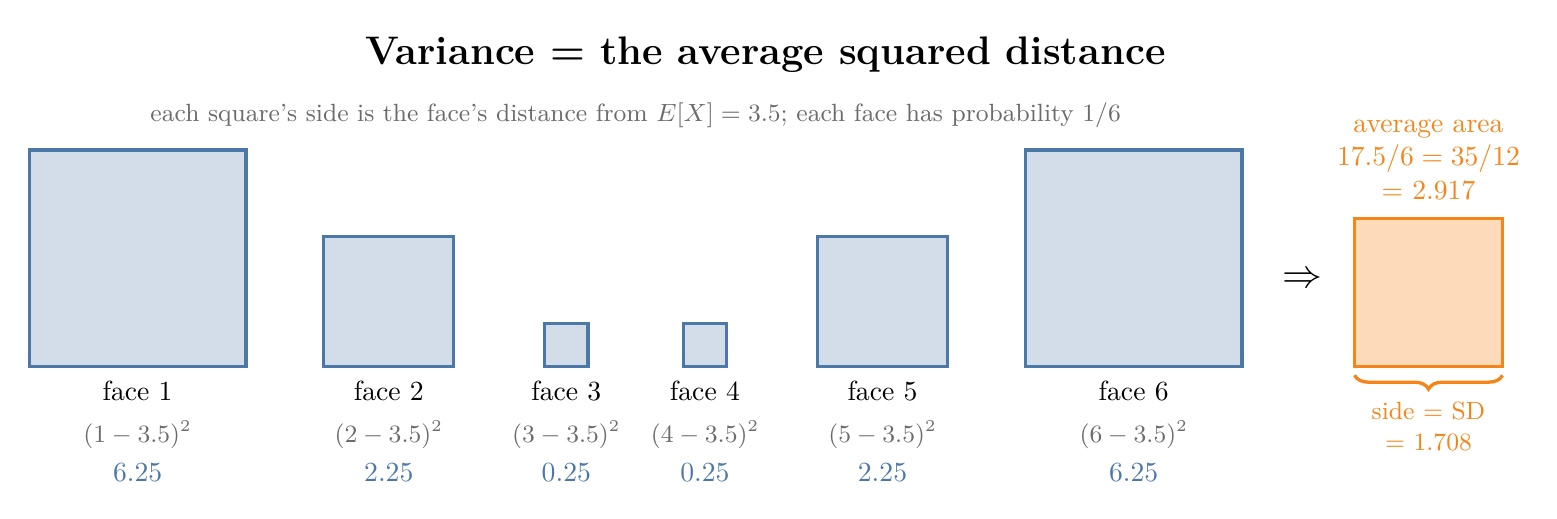
\begin{tikzpicture}[x=1.1cm, y=1.1cm]
  \node[title] at (8.5,3.6) {Variance = the average squared distance};
  \foreach \f in {1,...,6} {
    \pgfmathsetmacro{\s}{abs(\f-3.5)}
    \pgfmathsetmacro{\a}{\s*\s}
    \pgfmathsetmacro{\c}{\f<3.5 ? 1 : 0}
    \pgfmathsetmacro{\x}{{1.25,4.15,6.2,7.8,9.85,12.75}[\f-1] - \s/2}   % slot centres keep the labels apart
    \fill[cblue!25, draw=cblue] (\x,0) rectangle ++(\s,\s);
    \node[anchor=north, font=\sffamily] at (\x+\s/2,-0.05) {face \f};
    \node[anchor=north, font=\sffamily\small, text=cgrey] at (\x+\s/2,-0.5) {$(\f - 3.5)^2$};
    \node[anchor=north, font=\sffamily\bfseries, text=cblue] at (\x+\s/2,-1.0) {\pgfmathprintnumber[fixed,precision=2,fixed zerofill]{\a}};
  }
  \node[font=\sffamily\Large] at (14.7,1) {$\Rightarrow$};
  \pgfmathsetmacro{\v}{(6.25+2.25+0.25+0.25+2.25+6.25)/6}
  \pgfmathsetmacro{\sd}{sqrt(\v)}
  \fill[corange!30, draw=corange] (15.3,0) rectangle ++(\sd,\sd);
  \draw[decorate, decoration={brace, amplitude=5pt, mirror}, draw=corange] (15.3,-0.1) -- ++(\sd,0)
    node[midway, below=6pt, font=\sffamily\small, text=corange, align=center] {side = SD\\ = \pgfmathprintnumber[fixed,precision=3]{\sd}};
  \node[anchor=south, font=\sffamily, text=corange, align=center] at (15.3+\sd/2,\sd+0.1)
    {average area\\ $17.5/6 = 35/12$\\ = \pgfmathprintnumber[fixed,precision=3]{\v}};
  \node[note] at (7,2.9) {each square's side is the face's distance from $E[X] = 3.5$; each face has probability $1/6$};
\end{tikzpicture}
\end{document}
